% Use custom color mediblue CMYK 1,0,0,0.3 for all blue elements. In RGB it is around 0,50,70 (0..100) or 0,126,178 (0..255).
\documentclass[portrait,final,a0paper,fontscale=0.320]{imiseposter}
\usepackage[T1]{fontenc}
\usepackage[utf8]{inputenc}
\usepackage[english]{babel}% change to ngerman for a German poster
\microtypecontext{spacing=nonfrench}
% Using biblatex and biber. It's more modern but takes more than twice as long to compile in my case. ****
% If you use biblatex, you need to comment and uncomment the marked statements in the references as well.
%\usepackage{csquotes}
%\usepackage[style=numeric,backend=biber]{biblatex}
%\addbibresource{poster.bib}
%*********************************************************************************************************
\usepackage{graphicx}
\usepackage{url}% do not use hyperref as its links are displaced with baposter because of the font scale 
\usepackage{booktabs}

% Select Font %%%%%%%%%%%%%%%%%%%%%%%%%%%%%%%%%%%%%%%
%\usepackage{helvet} % closest to arial
\usepackage{bookman} % has some resemblance to Futura
%%%%%%%%%%%%%%%%%%%%%%%%%%%%%%%%%%%%%%%%%%%%%%%%%%%%%
\renewcommand{\familydefault}{\sfdefault}

\newcommand{\captionfont}{\footnotesize}
\usepackage[font=small,labelfont=bf]{caption}

\usepackage{tcolorbox}
\newtcolorbox{subsectionbox}[1]
{
  colframe=white,
  colback=white,
  colbacktitle=mediblue,
  sharp corners=all,
  title    = {#1},
}
\begin{document}

\begin{poster}% Set grid to false for final print
  {grid=true,}
  % Eye Catcher
  {}
  % Title
  {Anthropological Notation Ontology}
  % Authors
  {Alexandr Uciteli, Andy Ludwig, Prof. Dirk Labudde\\Konrad Höffner, Marie Heuschkel, Marleen Mohaupt}
  %{Alexandr Uciteli, Konrad Höffner{\small <konrad.hoeffner@imise.uni-leipzig.de>}, Andy Ludwig, other Author, Another Author}
  % University logo
  {% The makebox allows the title to flow into the logo, this is a hack because of the L shaped logo.
    %\includegraphics[height=9.0em]{img/medfak.pdf}
  }

%%%%%%%%%%%%%%%%%%%%%%%%%%%%%%%%%%%%%%%%%%%%%%%%%%%%%%%%%%%%%%%%%%%%%%%%%%%%%%
\begin{posterbox}[name=background,column=0,row=0]{Hintergrund}
Ziel ist die Entwicklung einer Ontologie für die einheitliche Einordnung von Knochenfunden aus Ausgrabungen in das Skelettsystem, die Beschreibung der Skelettstücke sowie die Definition von Funktionen zur Ableitung verschiedener Phänotypen des Menschen. 
\end{posterbox}
%%%%%%%%%%%%%%%%%%%%%%%%%%%%%%%%%%%%%%%%%%%%%%%%%%%%%%%%%%%%%%%%%%%%%%%%%%%%%%
\begin{posterbox}[name=ontology,below=background]{Ontologie}
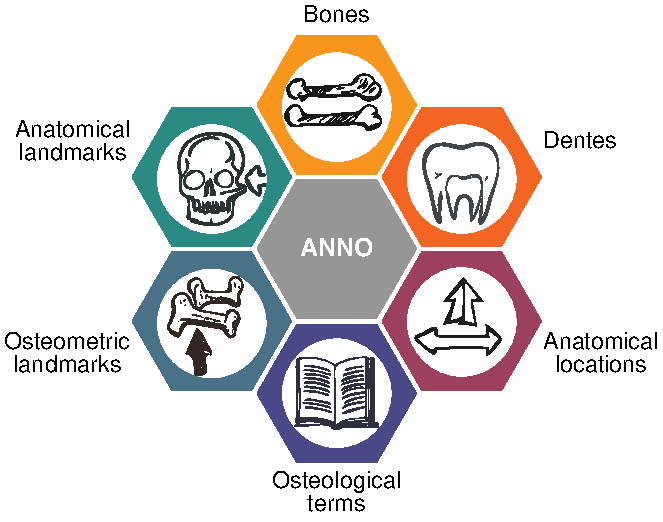
\includegraphics[width=\textwidth]{img/anno.pdf}
\begin{tabular}{ll}
\toprule
\textbf{Modul}			&\textbf{Inhalt}\\
\midrule
bones					&Knochen\\
dentes					&Zähne\\
anatomical locations	&Lage- und Richtungsbezeichnungen\\
osteological terms		&Begriffe zur Beschreibung des Skelettsystems\\
osteometric landmarks	&vordefinierte Punkte auf Skelettelementen\\
anatomical landmarks	&anatomische Punkte und Strukturen\\
\bottomrule
\end{tabular}

\begin{subsectionbox}{OLS~\cite{ols}~\small\url{https://ols.imise.uni-leipzig.de/ontologies/anno}}
\begin{itemize}
\item Visualisierungen der Beziehungen zwischen Klassen
\item Synchronisation mit NFDI über API
\item Download in Semantic-Web-Standardformaten
\end{itemize}

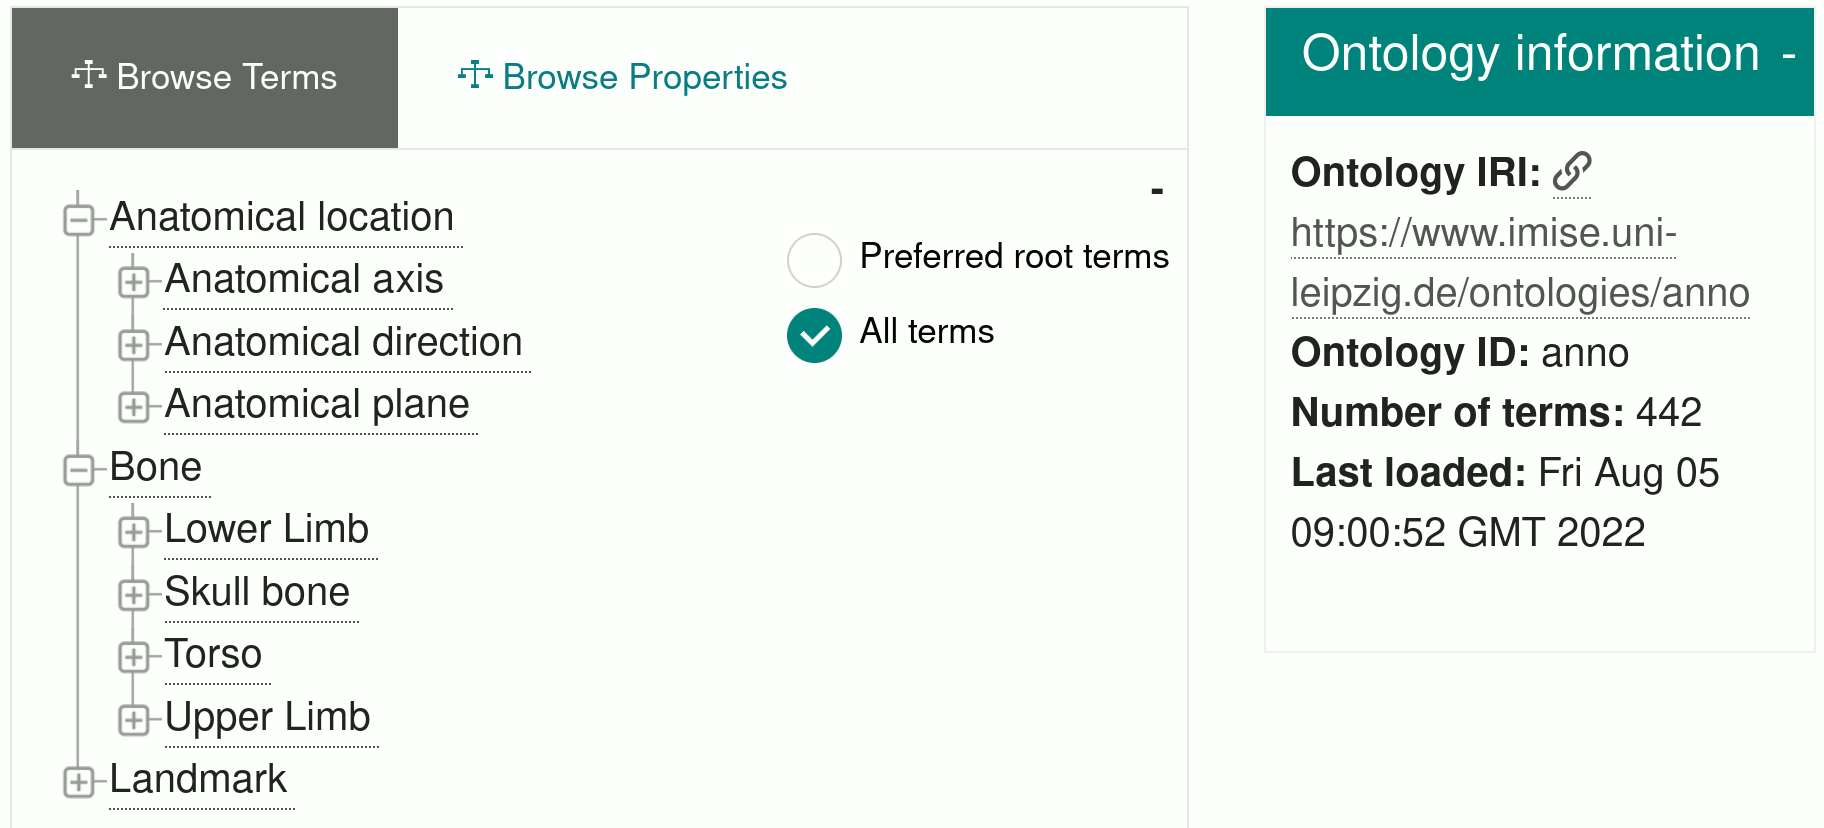
\includegraphics[width=\textwidth]{img/ols.png}
\end{subsectionbox}

\end{posterbox}
%%%%%%%%%%%%%%%%%%%%%%%%%%%%%%%%%%%%%%%%%%%%%%%%%%%%%%%%%%%%%%%%%%%%%%%%%%%%%%
\begin{posterbox}[name=results,column=1]{Mittweida}
Dieser Text ist ein Platzhalter für die Inhalte aus Mittweida

\begin{itemize}
\item Übertragung anthropologischer Untersuchungen in den digitalen Raum~\cite{digitalisierung}
\item Vorteile wie Sammlungsverknüpfung~\cite{spurensuche} und Standortunabhängigkeit, Materialerhalt 
\item Ontologie als Basis (Start mit Festlegung einer einheitlichen anatomischen Landkarte, Möglichkeit der Automatisierung bei Messungen, dadurch Möglichkeit mehr Messungen / Daten aufzunehmen) für Digitale Speicherung und Verknüpfung anthropologischer Informationen 
Ermöglicht weitergehende Analysen und Untersuchungsprozesse 
\end{itemize}
dieses bild kommt noch nach links\\
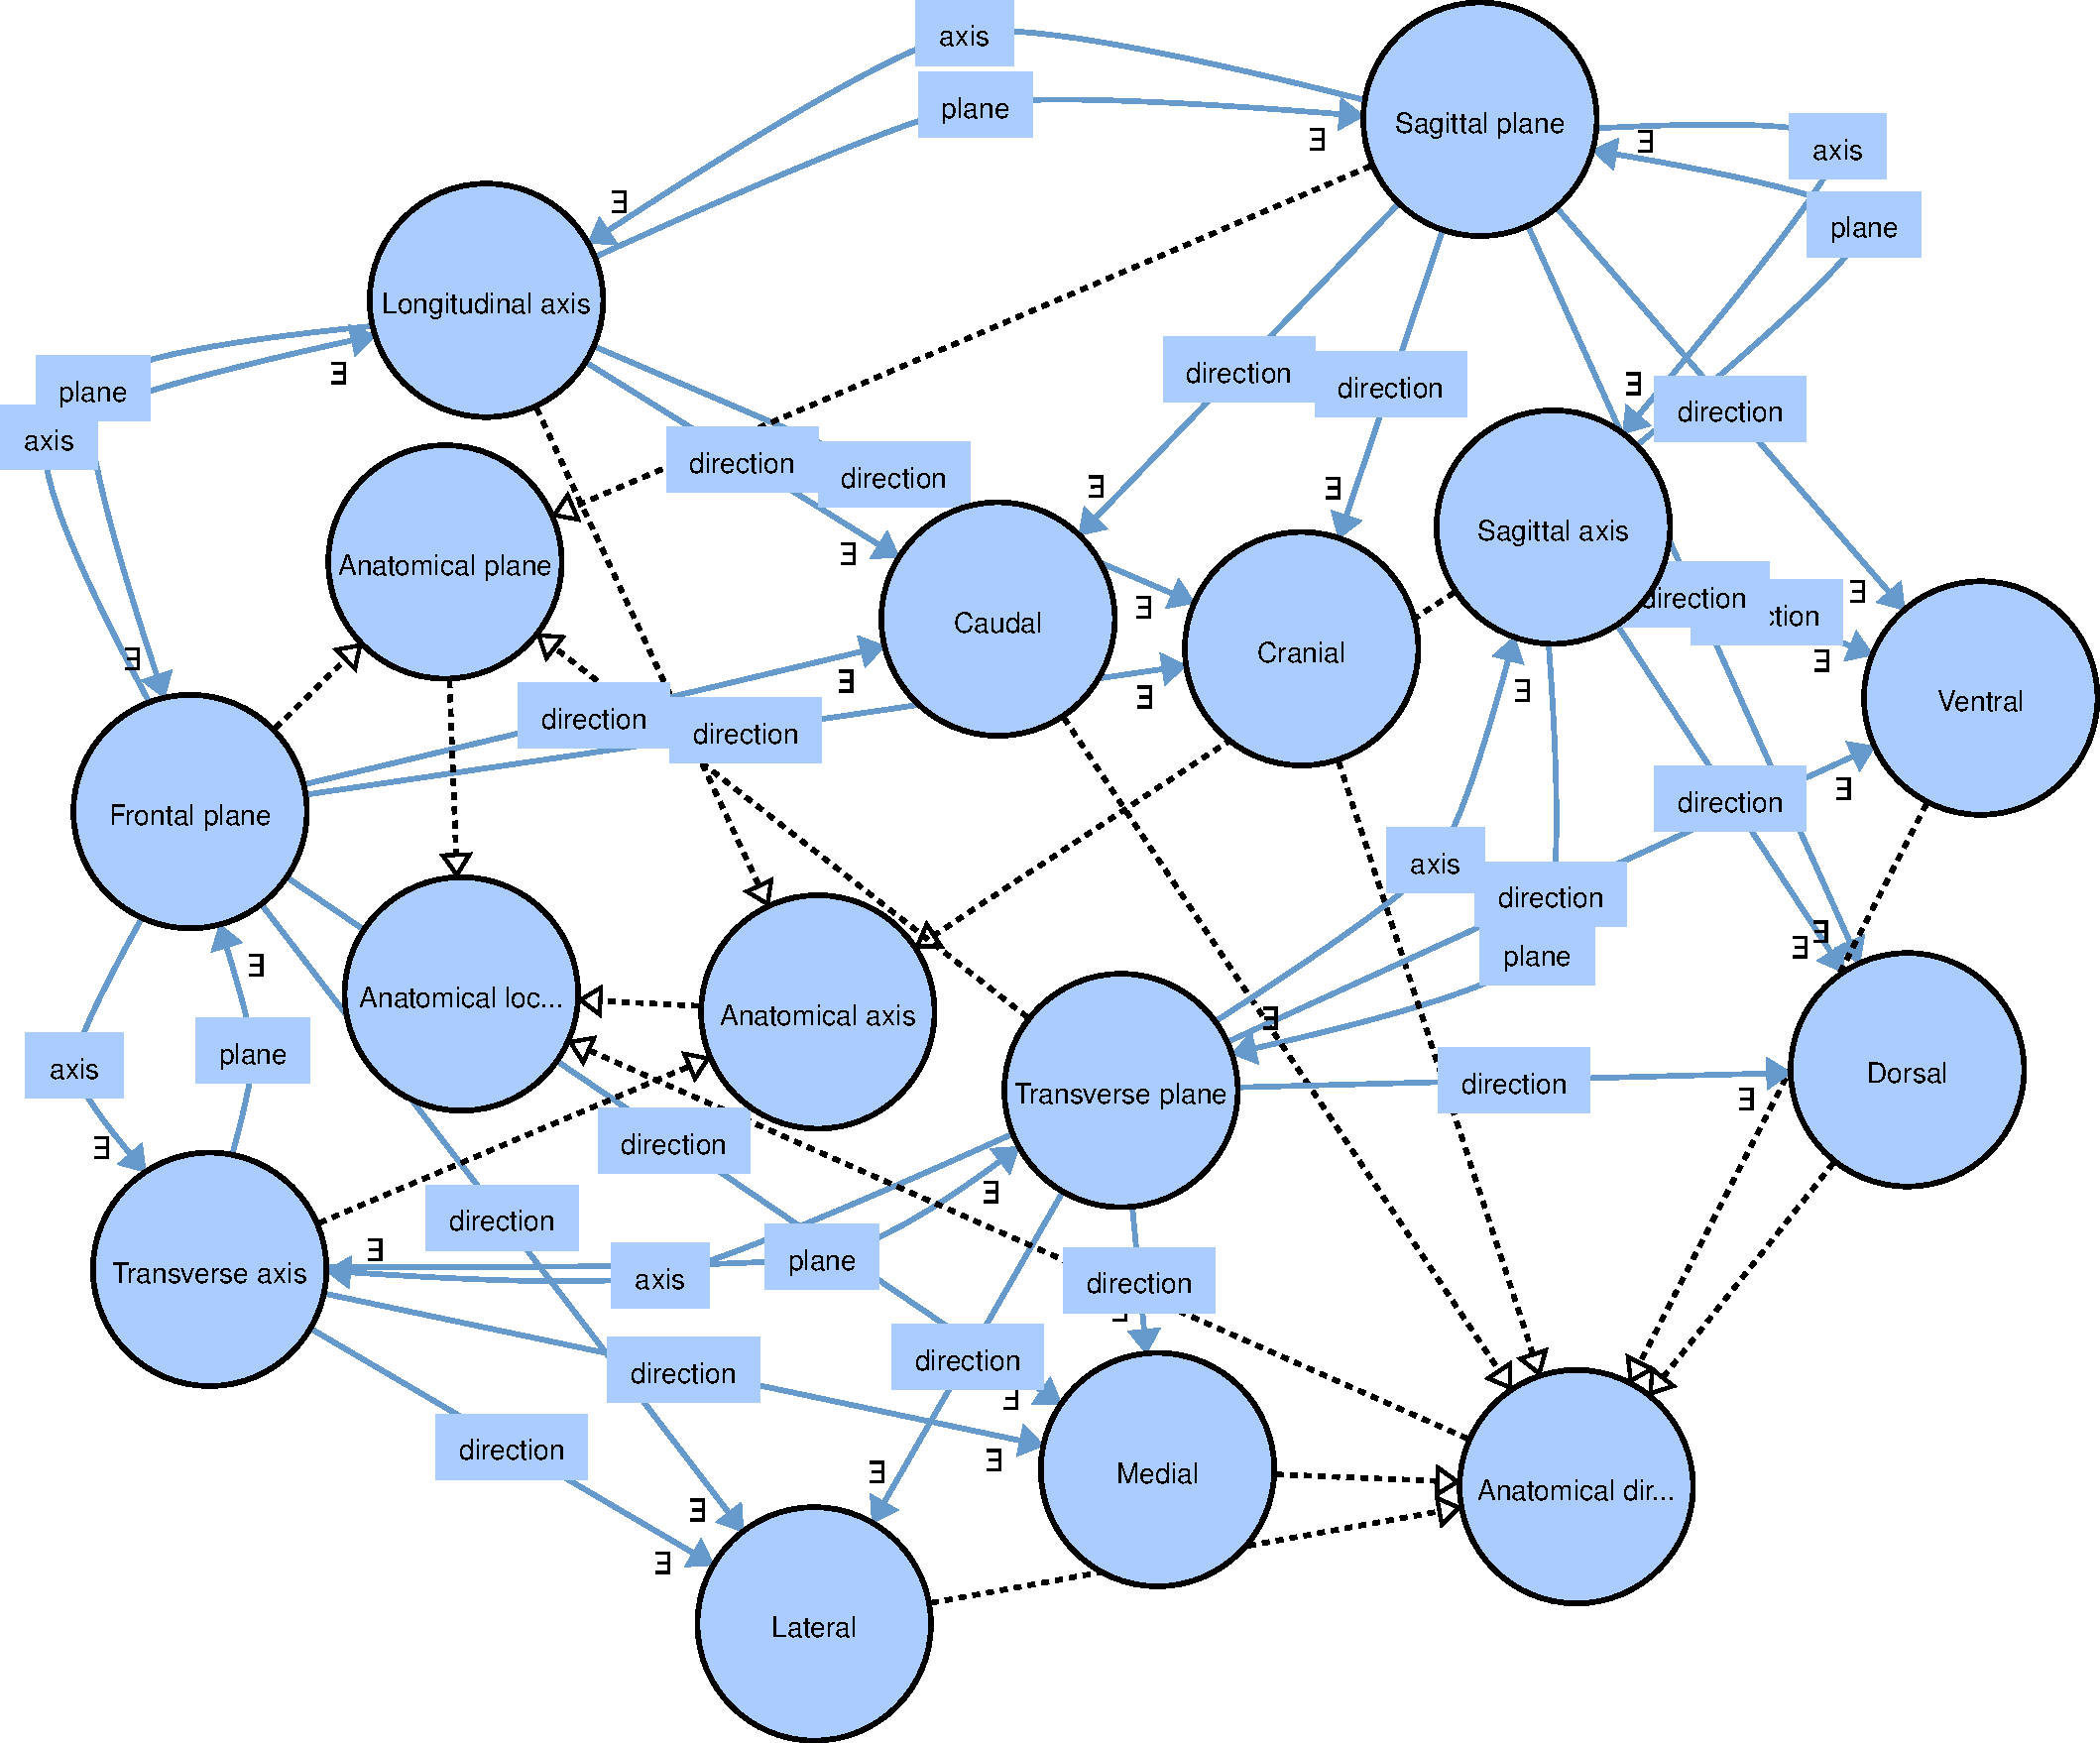
\includegraphics[width=0.8\textwidth]{img/location.pdf}
\end{posterbox}
%%%%%%%%%%%%%%%%%%%%%%%%%%%%%%%%%%%%%%%%%%%%%%%%%%%%%%%%%%%%%%%%%%%%%%%%%%%%%%
%\begin{posterbox}[name=discussion,column=1,below=results]{Discussion}
%\end{posterbox}
%%%%%%%%%%%%%%%%%%%%%%%%%%%%%%%%%%%%%%%%%%%%%%%%%%%%%%%%%%%%%%%%%%%%%%%%%%%%%%
\begin{posterbox}[name=references,column=0,below=ontology]{References}
    \small
    \begingroup
    \renewcommand{\section}[2]{}%suppress heading
    % using bibtex ***********
    \bibliographystyle{abbrvdin}
    \bibliography{anno}
    % using biblatex *********
    %\printbibliography
    %*************************
    \endgroup
    \vspace{0.3em}
  \end{posterbox}
%%%%%%%%%%%%%%% Anno Logo
 \node [anchor=south east, inner sep=1pt,xshift=14em,yshift=-14em] at (current page.north west)
 {
\includegraphics[height=0.105\textheight]{img/anno-logo-short-mediblue.pdf}};
%%%%%%%%%%%%%%%  Founded by SaxFDM, their guidelines say to use the Saxony signet
 %\node [anchor=south east, inner sep=1pt,xshift=-3.5em] at (current page.south east) % for unknown reasons the xshift is necessary
 \node [anchor=south east, inner sep=1pt,xshift=-8.5em,yshift=-13em] at (current page.north east) % for unknown reasons the xshift is necessary
 %{\includegraphics[height=0.03\textheight]{img/dfg-logo.pdf}
 {
\includegraphics[height=0.08\textheight]{img/sachsen-signet.pdf}};
%%%%%%%%%%%%%%% Medical Faculty Logo
 \node [anchor=south east, inner sep=1pt,xshift=-17em,yshift=-2em] at (current page.south east)
 {\includegraphics[height=4cm,decodearray=0 0 0 0 0 1]{img/medfak.pdf}};
%%%%%%%%%%%%%%% Hochschule Mittweida
 \node [anchor=south east, inner sep=1pt,xshift=-19em,yshift=8em] at (current page.south east)
 {
\includegraphics[height=2.2cm]{img/mittweida-logo-mediblue.pdf}};
%%%%%%%%%%%%%%% FoSIL
 \node [anchor=south east, inner sep=1pt,xshift=-3.5em,yshift=7.9em] at (current page.south east)
 {
\includegraphics[height=2.2cm]{img/fosil-logo.png}};
%%%%%%%%%%%%%%% IMISE Logo
 \node [anchor=south east, inner sep=1pt,xshift=-3em,yshift=2em] at (current page.south east)
 {
\includegraphics[height=1.5cm]{img/imise-logo.pdf}};
%%%%%%%%%%%%%%%%%%%%%%%%%%%%%%%%%%%%%%%%%%%%%%%%%%%%%%%%%%%%%%%%%%%%%%%%%%%%%%
\end{poster}
\end{document}
